\documentclass[aspectratio=169]{beamer}
\usetheme{metropolis}

\usepackage[utf8]{inputenc}
\usepackage[OT4]{polski}
\usepackage{flexisym}
\usepackage{parskip}
\usepackage{algpseudocode,amsmath}
\newcommand{\var}{\texttt}
\newcommand{\assign}{\leftarrow}

\usepackage{listings}
\usepackage{color}

\usepackage{capt-of}


\definecolor{dkgreen}{rgb}{0,0.6,0}
\definecolor{gray}{rgb}{0.5,0.5,0.5}
\definecolor{mauve}{rgb}{0.58,0,0.82}

\lstset{frame=tb,
	language=c++,
	aboveskip=3mm,
	belowskip=3mm,
	showstringspaces=false,
	columns=flexible,
	basicstyle={\small\ttfamily},
	numbers=none,
	numberstyle=\tiny\color{gray},
	keywordstyle=\color{blue},
	commentstyle=\color{dkgreen},
	stringstyle=\color{mauve},
	breaklines=true,
	breakatwhitespace=true,
	tabsize=3
}


\title{Zadanie 10. Podział liczby}
\subtitle{Adrian Rupala}

\begin{document}
	\frame {
		\titlepage
	}

	\frame {
		\frametitle{Treść zadania}
		\fontsize{10pt}{7.2}\selectfont
		Liczbę naturalną $C$ można przedstawić jako sumę parami różnych liczb naturalnych. \\Na przykład jeśli $C = 6$, to możemy C przedstawić na cztery sposoby:
		\\$1+2+3$
		\\$1+5$
		\\$2+4$
		\\$6$ 
		\\a jeśli $C = 10$, to takimi podziałami są:
		\\$1+2+3+4$
		\\$1+2+7$
		\\$1+3+6$
		\\$1+4+5$
		\\$1+9$
		\\$2+3+5$
		\\$2+8$
		\\$3+7$
		\\$4+6$
		\\$10$
		\\Skonstruuj algorytm wyczerpujący z nawrotami, generujący wszystkie podziały podanej liczby naturalnej $C$.~
	}

	\frame{
		\frametitle{Definicje}
		\fontsize{14pt}{7.2}\selectfont
		\large Algorytm z nawrotami (backtracking) - algorytm wyszukiwania wszystkich lub kilku rozwiązań polegający na znajdowaniu wyniku metodą "prób i błędów", wszelako z oznaczeniem niepowodzeń, dzięki czemu te same błędy nie są popełniane dwukrotnie. ~ \bigskip
			
		\large Jeżeli problem pozwala na zastosowanie algorytmu wyszukiwania z nawrotami, to metoda ta może być znaczenie efektywniejsza niż wyszukiwanie wyczerpujące (zakładając przeszukiwanie wszystkich rozwiązań), ponieważ pojedynczy test może wyeliminować nie jedno a wiele rozwiązań niedopuszczalnych. ~
	}

	\frame{
	\frametitle{Definicje}
	\fontsize{14pt}{7.2}\selectfont
	\large Rekurencja - technika programowania, dzięki której funkcja, procedura lub podprogram jest w stanie w swoim ciele wywołać sam siebie. Pozwala ona łatwo wykonać wiele zadań, w których potrzeba jest wyników cząstkowych do obliczenia całości. ~
		
	}

	\begin{frame}[fragile]
	\frametitle{Rozwiązanie - pseudokod}

			\begin{lstlisting}
			void sprawdz_i_wypisz(int pozycja, int pozostalo) {
				if (pozostalo == 0 && znajdzDuplikat(lista, pozycja) == false) {
					for (int i = 1; i <= pozycja - 1; i++) {
						cout << lista[i] << " ";
					}
					cout << endl;
				} else {
					for (int k = lista[pozycja - 1]; k <= pozostalo; k++) {
						lista[pozycja] = k;
						sprawdz_i_wypisz(pozycja + 1, pozostalo - k);
					}
				}
			}			
			\end{lstlisting}

	\end{frame}

		\begin{frame}[fragile]
		\frametitle{Rozwiązanie - pseudokod}
	
		\begin{lstlisting}
			
		void wywolanie(int C) {
			lista[0] = 1;
			sprawdz_i_wypisz(1, C);
		}
		\end{lstlisting}
	
	\end{frame}

	\begin{frame}[fragile]
	\frametitle{Rozwiązanie - pseudokod}
			
			\begin{lstlisting}
				bool znajdz_duplikat(int lista[], int rozmiar_tablicy) {
					sort(lista);
					for (int i = 0; i < rozmiar_tablicy - 1; i++) {
						if (lista[i] == lista[i + 1]){
							return true;
						}
					}
					return false;
				}
			\end{lstlisting}
			
	\end{frame}

	\begin{frame}[fragile]
	\frametitle{Wykonanie kodu}
		\begin{columns}
			\column{.5\textwidth}
			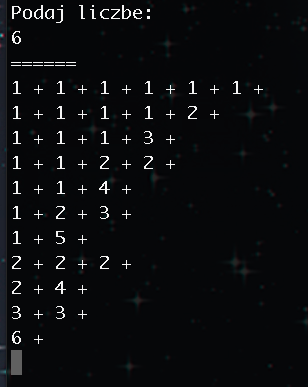
\includegraphics[width=\columnwidth]{source/1.png}
			\captionof{figure}{Wynik dla liczby 6 z powtórzeniami.}
			
			\column{.5\textwidth}
			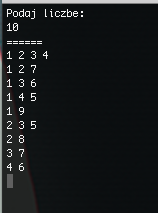
\includegraphics[width=\columnwidth]{source/2.png}
  			\captionof{figure}{Wynik dla liczby 6 bez powtórzeń.}

		\end{columns}
	\end{frame}

	\begin{frame}[fragile]
	\frametitle{Wykonanie kodu}
		\begin{columns}
			\column{.5\textwidth}
			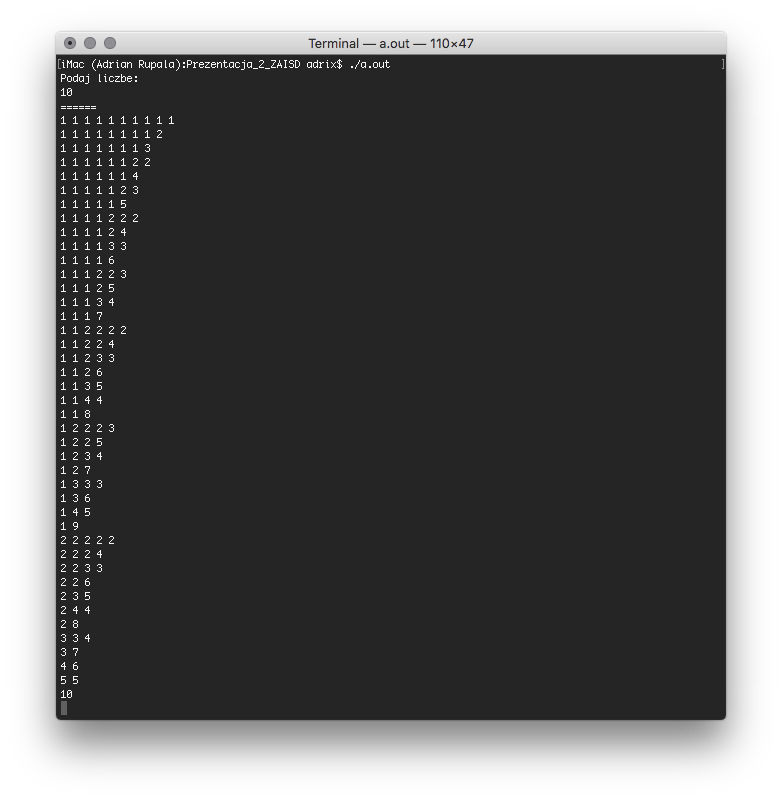
\includegraphics[width=\columnwidth,height=140px]{source/3.png}
			\captionof{figure}{Wynik dla liczby 10 z powtórzeniami.}
			
			\column{.5\textwidth}
			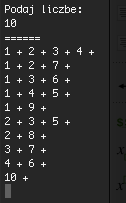
\includegraphics[width=\columnwidth]{source/4.png}
			\captionof{figure}{Wynik dla liczby 10 bez powtórzeń.}
			
		\end{columns}
	\end{frame}
	
		
	\frame{
		\centering \Huge
		\emph{Dziękuję za uwagę!}
	}
	
\end{document}
